% OVERVIEW
We will now apply the inferential machinery of multilevel calibration for solving the Bayesian interpretation of the uncertainty characterization subproblem A of the NASA Langley multidisciplinary UQ challenge.
The problem will be solved in its original formulation involving ``perfect'' data.
% INDEPENDENCE SAMPLER
Motivated by findings from first preliminary problem analyses, posterior densities of the QoI will be computed by a suitable MH independence sampler.
% HARDWARE ARCHITECTURE & SOFTWARE ENVIRONMENT
This sampler will be implemented in MATLAB and serially run on a modern CPU.
Nevertheless we will discuss possible parallelization strategies.
% DATA CONFIGURATIONS
The total data \(\tuple{\perfect{y}_i}_{1 \leq i \leq 50}\) and its subconfigurations \(\tuple{\perfect{y}_i}_{1 \leq i \leq 25}\)
and \(\tuple{\perfect{y}_i}_{26 \leq i \leq 50}\) will be analyzed with the devised algorithm.
% POSTERIOR FIDELITY
Based on heuristic parameter tuning and plausibility checks we will assess the fidelity of the posterior.
% DATA AUGMENTATION
Promising a boost of posterior fidelity we will lastly devise a hybrid MCMC scheme which is based on data augmentation and both independence and random walk sampling.

\subsection{Preliminary analyses}
% SIGNIFICANCE OF BASIC INSIGHT
A basic understanding of an inverse problem under consideration allows to judge the performance of various potential MCMC schemes.
This allows to design efficient algorithms and it is indispensable since it prevents from obtaining misleading results that are due to inappropriate samplers.
% MCMC
In order to gain first insights into the present multilevel calibration problem, we perform a number of initial MCMC runs that were based on crude random walk Metropolis sampling.
Thereby we could provisionally assess the principal nature of the posteriors \cref{eq:JAIS:Multilevel:Posterior,eq:JAIS:PerfectData:Posterior}.
% MAIN FINDINGS: PUSH-FORWARD
Main findings from sampling the posterior \cref{eq:JAIS:PerfectData:Posterior} indicate that posterior marginals of the QoI
\((p_2,\bm{\theta}_1,\bm{\theta}_{45})\) may very well be multimodal or broad distributions that significantly overlap with the marginal priors.
\par % MAIN FINDINGS: JOINT POSTERIOR
Solving a joint problem in the presence of additional measurement noise provides further insight.
Notwithstanding that this is actually a different problem, it will eventually prove valuable.
Sampling the joint posterior \cref{eq:JAIS:Multilevel:Posterior} of the entirety of unknowns \((\tuple{p_{1,i}},p_2,\tuple{p_{3,i}},\tuple{p_{4,i}},\tuple{p_{5,i}},\bm{\theta}_1,\bm{\theta}_{45})\)
reveals further information about the unknowns, e.g.\ it occurs that experiment-specific unknowns \(\tuple{p_{1,i}}\) are identifiable and their posterior marginals feature single modes.
% ADDED EXPLANATION
This does not refer to the posteriors of \(\tuple{p_{3,i}}\) and \(\tuple{p_{4,i}}\) that are rather flat and the ones of \(\tuple{p_{5,i}}\) that are bimodal.
% CONCLUSION
Altogether those preliminary analyses have provided useful information that will eventually motivate the final MCMC samplers.

\subsection{``Perfect'' data analysis}
For the calibration of the  Bayesian multilevel model \cref{eq:JAIS:PerfectData:Model} we devise a blockwise independence MCMC sampler.
Since the algorithm is based on MCMC, MC and KS techniques, hereinafter it will be referred to as \(\text{MC}^3\text{KS}\).
QoI are grouped in blocks \((p_2)\), \((\mu_1,\sigma^2_1)\), \((\mu_4,\sigma^2_4,\rho_{45})\) and \((\mu_5,\sigma^2_5)\)
that are consecutively updated by sampling blockwise candidates from the corresponding prior distributions.
% PRIOR SAMPLING
In many cases independence sampling from the priors is inefficient due to a negligible overlap between the prior and the posterior distributions and the resulting low acceptance rates.
However, on account of the multimodality of the posteriors and their overlap with the priors, that were indicated by first analyses, independence sampling promises rapid mixing for the problem at hand.
\par % FIDELITY
Moreover in the context of \cref{eq:JAIS:MCMC:LikelihoodRatio} we suppose that wide jumps in the parameter space, that are induced by independence sampling on average, are beneficial in terms of posterior fidelity.
% ADDED EXPLANATION
For wide jumps the difference of the likelihood at the current and the candidate state of the Markov chain tends to be larger than for small jumps.
Following previous discussions, to some extent this alleviates the error statistics of repeated likelihood estimations for the same state.
% ADVANTAGE
Another advantage of the devised MCMC scheme over random walk sampling is that apart from its blockwise updating structure, it does not require extensive fine-tuning of the proposal distribution.
% BLOCKWISE SAMPLING
Updating in blocks intents to minimize the number of calls to the likelihood \cref{eq:JAIS:PerfectData:KernelSmoothedLikelihood}
that are necessary for each block in each MCMC iteration, while maintaining high acceptance rates that are favorable for independence sampling.
% BETA DISTRIBUTION
With the help of \cref{eq:JAIS:Beta:Transform2Shape} the constraints \(\alpha_1,\beta_1>1\) are enforced by rejecting nonconforming proposals in the block \((\mu_1,\sigma^2_1)\).
% INITIALIZATION
The \(\text{MC}^3\text{KS}\) sampler is initialized by setting parameters in the middle of their admissible intervals.
Due to rapid mixing the initialization is not of crucial importance for the employed sampling scheme.
% GENERAL EXPECTATIONS
Generally speaking we expect that forward model parameters and mean hyperparameters are easier to identify than spread or even correlation hyperparameters.

\subsection{Likelihood estimation and posterior fidelity} \label{sec:JAIS:Analysis:LikelihoodEstimation}
% GAUSSIAN KERNEL
For the estimation \cref{eq:JAIS:PerfectData:KernelSmoothedLikelihood} of the transformed likelihood \cref{eq:JAIS:PerfectData:Likelihood} we choose kernel functions \(\mathcal{K}\) of Gaussian type.
% TUNING HEURISTICS
In order to achieve a convenient trade-off between the conflicting endeavors fidelity of the posterior and ease of its computation, the number of samples \(K\) and the bandwidth \(h\) have to be set.
% COMPUTATIONAL LIMITATIONS
In practice computational resource limitations restrict the total number of affordable forward model runs, hence we approach parameter tuning from the situation of a given \(K\).
\par % CASCADE OF RUNS
Owing to the absence of a rigorous means to define a corresponding and ``optimal''  bandwidth \(h\), we study the posteriors obtained for fixed \(K=10^4\) and decreasing \(h\) in a cascade of runs.
% SHRINKAGE & COLLAPSE
We observe an initial shrinkage of the posterior, i.e.\ evolving from the flat prior it takes on definite shape, and an eventual collapse, i.e.\ the posterior flattens out again and looses its structure.
The initial shrinkage is associated with significant changes of the posterior shape, the eventual breakdown is QoI-dependent, and in between the posterior is relatively stable with respect to \(h\).
% EXPECTATION
We remark that this behavior is consistent with \cref{eq:JAIS:MCMC:MHCorrection,eq:JAIS:MCMC:LikelihoodRatio}.
Significant oversmoothing the target density \cref{eq:JAIS:PerfectData:PushForwardDensity}, i.e.\ a strongly biased estimator \cref{eq:JAIS:PerfectData:KernelSmoothedLikelihood},
can falsely assign posterior mass to QoI-values that do not well-explain or even contradict the data.
Considerable undersmoothing of the target density, i.e.\ a high variance of the estimator \cref{eq:JAIS:PerfectData:KernelSmoothedLikelihood}, can cause ``arbitrary'' acceptances in the MH correction.
% POSTERIOR FIDELITY
We speculate that in between those extremes, the more stable the posterior is with respect to small changes in \(h\), the more confident we can be to have revealed the true posterior.
% DINSTINCTIVENESS
Beyond that we presume that a high degree of distinctiveness of the posterior with respect to the prior indicates high posterior fidelity.
The converse statement does not hold, though.
\par % PLAUSIBILITY CHECK
In addition to those heuristics we perform a plausibility check as follows.
% ``IMPERFECT'' DATA
During preliminary analysis we have solved the UQ challenge problem in the presence of additional measurement noise \(\varepsilon_i\) with \(E_i \sim \mathcal{N}(\varepsilon_i \cond 0,\sigma^2_i)\),
i.e.\ we sampled a joint posterior of the form \cref{eq:JAIS:Multilevel:Posterior}.
If the corresponding noise-level \(\sigma^2_i\) tends to zero the results of analyzing ``imperfect'' data should approach the ones of analyzing ``perfect'' data.
Indeed we find that for low levels of noise \(\sigma^2_i \gtrsim 0\) the joint problem solution resembles our final results for analyzing ``perfect'' data.
While the posterior \cref{eq:JAIS:PerfectData:Posterior} can only be approximately explored with the dubious aid of statistical likelihood estimations
\cref{eq:JAIS:PerfectData:KernelSmoothedLikelihood}, the joint posterior \cref{eq:JAIS:Multilevel:Posterior} can be sampled exactly.
Thus we have found that our approximate solution to the actual problem reminds of an exact solution to an only slightly different problem.
For ``well-behaved'' problems we take this observation as an indication of an acceptable degree of posterior fidelity.
\par % LIKELIHOOD ESTIMATION
% PARAMETERS
Following this discussion \(K=10^4\) and \(h=0.002\) constitutes our final parameter setup.
% FIGURE
The principle of estimating the density \cref{eq:JAIS:PerfectData:PushForwardDensity} and the transformed likelihood \cref{eq:JAIS:PerfectData:Likelihood} is visualized in \cref{pre:JAIS:TransformedLikelihood}.
Samples of \(K=10^4\) and \(K=10^7\) forward model responses are simulated for two different (hyper)parameter values
\((p_2,\bm{\theta}_1,\bm{\theta}_{45})_{\mathrm{high}}\) and \((p_2,\bm{\theta}_1,\bm{\theta}_{45})_{\mathrm{low}}\).
As judged from our final results, these are (hyper)parameter values of high and low degree of posterior evidence, respectively.
For the smaller sample with \(K=10^4\) estimates of the sought densities \(f(\perfect{y}_i \cond p_2,\bm{\theta}_1,\bm{\theta}_{45},\bm{\theta}_3)\) are shown.
For reference purposes a histogram of the larger sample with \(K=10^7\) is shown.
% PROBLEM CHARACTER
It can be seen that response densities \(f(\perfect{y}_i \cond p_2,\bm{\theta}_1,\bm{\theta}_{45},\bm{\theta}_3)\)
for \((p_2,\bm{\theta}_1,\bm{\theta}_{45})_{\mathrm{high}}\) and \((p_2,\bm{\theta}_1,\bm{\theta}_{45})_{\mathrm{low}}\) significantly overlap.
This is a problem characteristic that complicates the statistical identification of the QoI \((p_2,\bm{\theta}_1,\bm{\theta}_{45})\).
% MC^3KS: EVALUATION OF THE TRANSFORMED LIKELIHOOD
\begin{figure}[htbp]
  \centering
  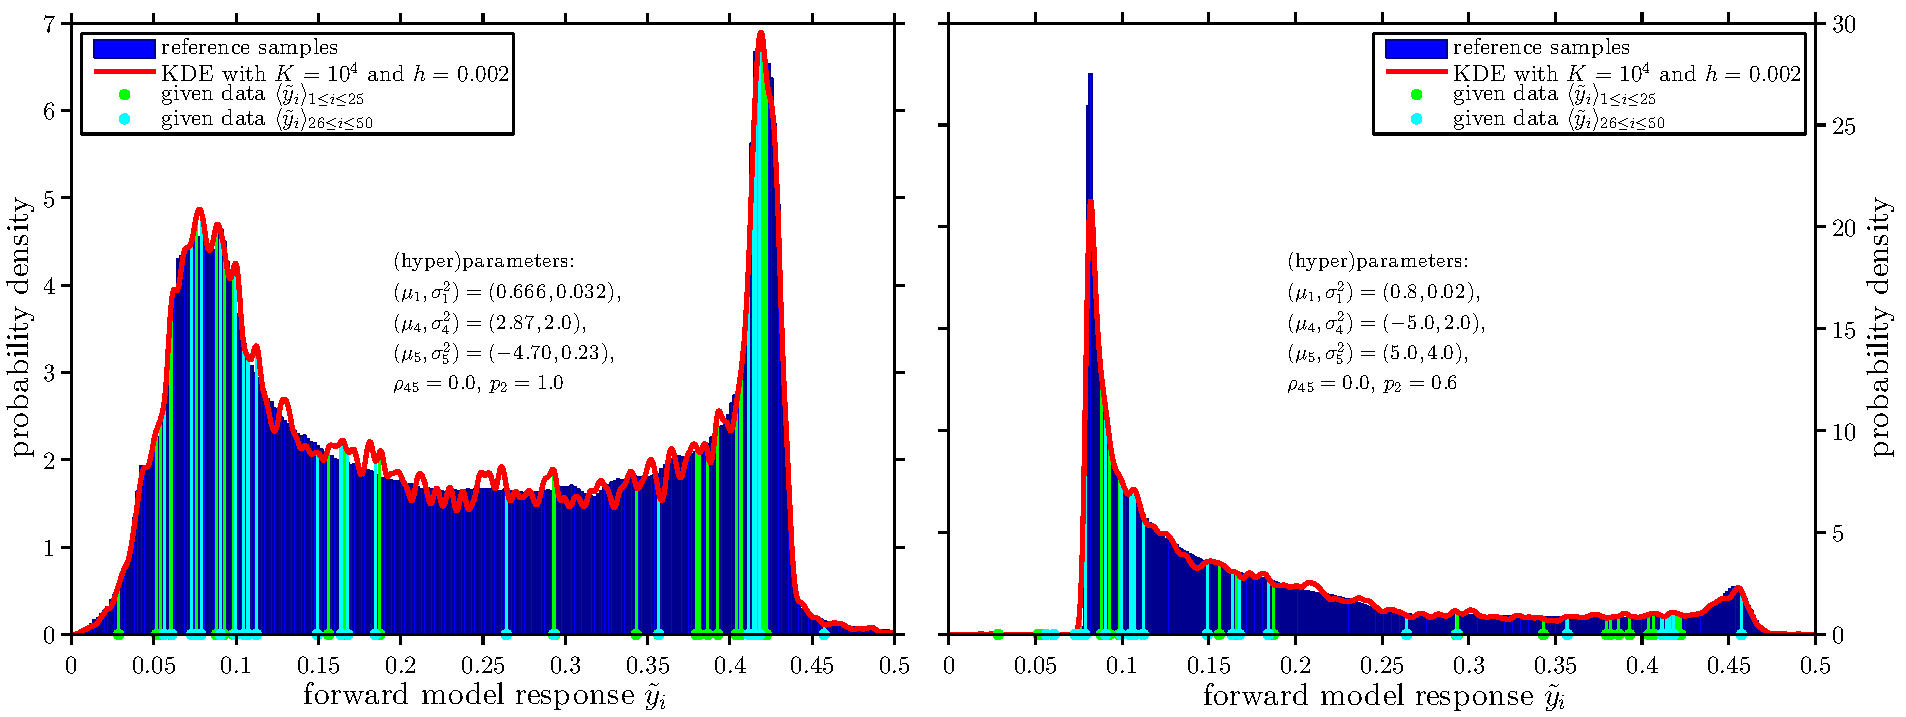
\includegraphics[width=\JAISfigWidth]{fig_JAIS_KS_TransformedLikelihood}
  \caption[Estimation of \(f(\perfect{y}_i \cond p_2,\bm{\theta}_1,\bm{\theta}_{45},\bm{\theta}_3)\)]{Estimation of \(f(\perfect{y}_i \cond p_2,\bm{\theta}_1,\bm{\theta}_{45},\bm{\theta}_3)\).
           Evaluating the transformed likelihood \cref{eq:JAIS:PerfectData:Likelihood} for \(\text{MC}^3\text{KS}\)
           is based on the forward model response density \cref{eq:JAIS:PerfectData:PushForwardDensity}.
           For two different values of the (hyper)parameters \((p_2,\bm{\theta}_1,\bm{\theta}_{45})\) a KDE of 
           \(f(\perfect{y}_i \cond p_2,\bm{\theta}_1,\bm{\theta}_{45},\bm{\theta}_3)\) with \(K=10^4\) and \(h=0.002\) is shown.
           Histograms with \(K=10^7\) forward model responses are shown as a reference.
          }
  \label{pre:JAIS:TransformedLikelihood}
\end{figure}
\par % UNDERSMOOTHING
It can also be seen that the employed bandwidth \(h=0.002\) amounts to a slight undersmoothing of the target density, i.e.\ a bias-variance trade-off favoring lower bias yet acceptable variance.
This is advantageous because it allows to capture local small-scale features of the target density, e.g.\ sharp peaks and edges, in the posterior.
% PSEUDO-MARGINAL
We remark that in the context of pseudo-marginal MCMC \cite{MCMC:Andrieu2009} this observation supports the speculation that it is preferable to minimize the bias in \cref{eq:JAIS:PerfectData:MSE}.
% AUTOMATIC BANDWIDTH SELECTION
Since the target density significantly differs from a normal distribution, automatic bandwidth selection cannot be based on the normal reference rule.
The resulting oversmoothing of the target density, i.e.\ a significantly biased KDE, would veil its important characteristics.
% SOLUTION FIDELITY
Finally the (hyper)parameter values \((p_2,\bm{\theta}_1,\bm{\theta}_{45})_{\mathrm{high}}\) can be seen to lead to a response density that explains the data sample \(\tuple{\perfect{y}_i}\) reasonably well.
% POSTERIOR FIGURES
% \mu_1, \sigma^2_1
\begin{figure}[p]
  \centering
  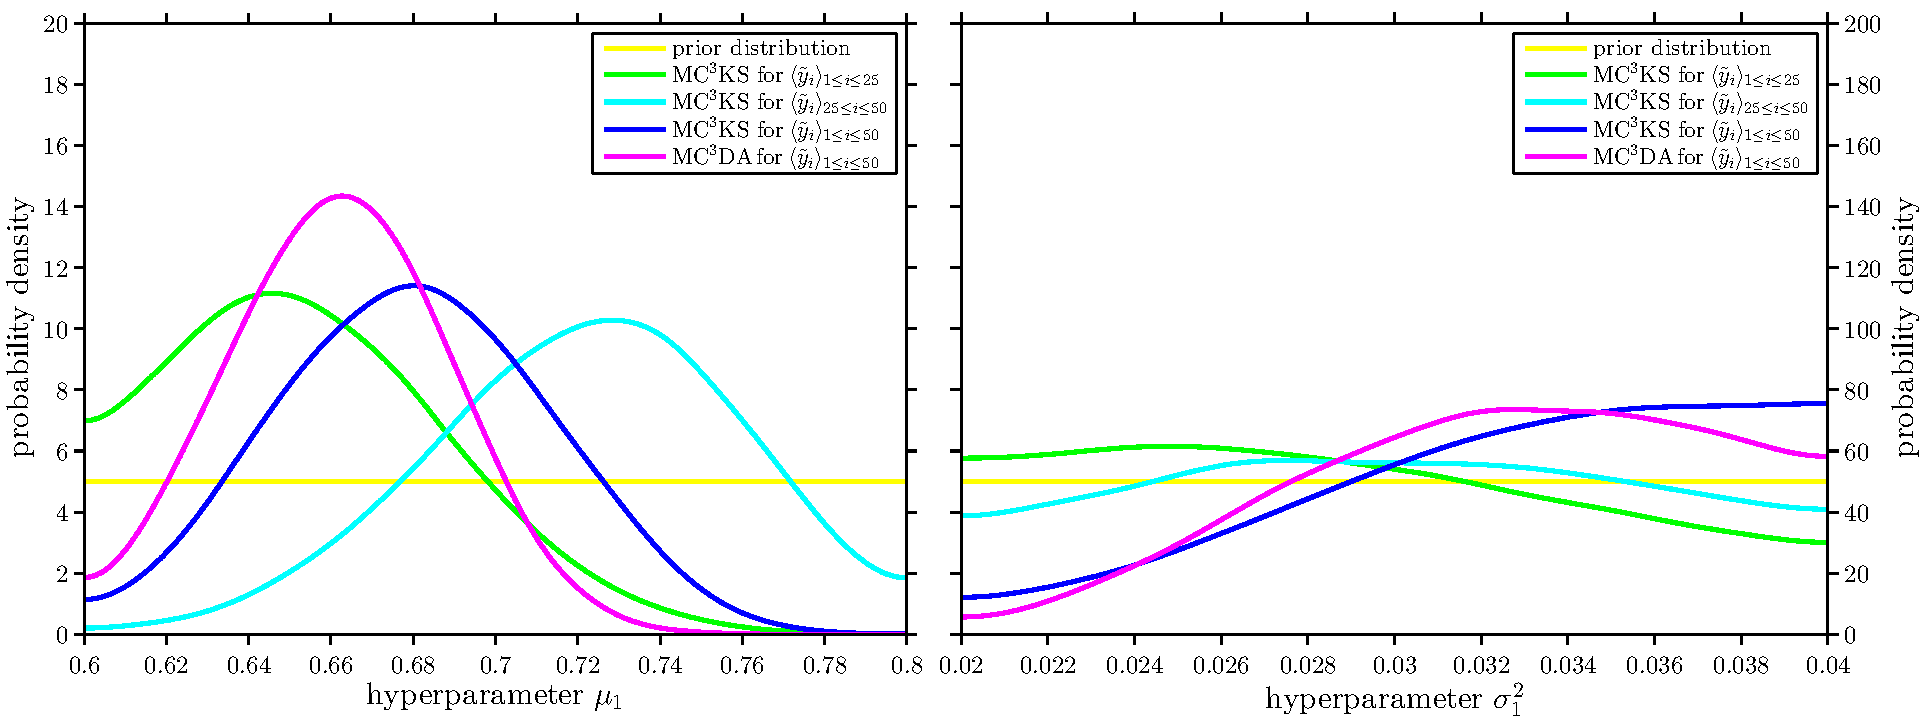
\includegraphics[width=\JAISfigWidth]{fig_JAIS_KSDA_1D_Hyper1}
  \caption[Posterior marginals of \(\mu_1\) and \(\sigma^2_1\)]{Posterior marginals of \(\mu_1\) and \(\sigma^2_1\).
           The posterior of \(\mu_1\) features a clear structure as compared to the prior.
           Separate analyses of \(\tuple{\perfect{y}_i}_{1 \leq i \leq 25}\) and \(\tuple{\perfect{y}_i}_{26 \leq i \leq 50}\) lead to different posterior modes,
           whereas jointly analyzing \(\tuple{\perfect{y}_i}_{1 \leq i \leq 50}\) leads to a mode in between the two aforementioned ones.
           The posterior marginal of \(\sigma^2_1\) is seen to be less informative.
          }
  \label{res:JAIS:Hyper1}
\end{figure}
% p_2 & \rho_{45}
\begin{figure}[p]
  \centering
  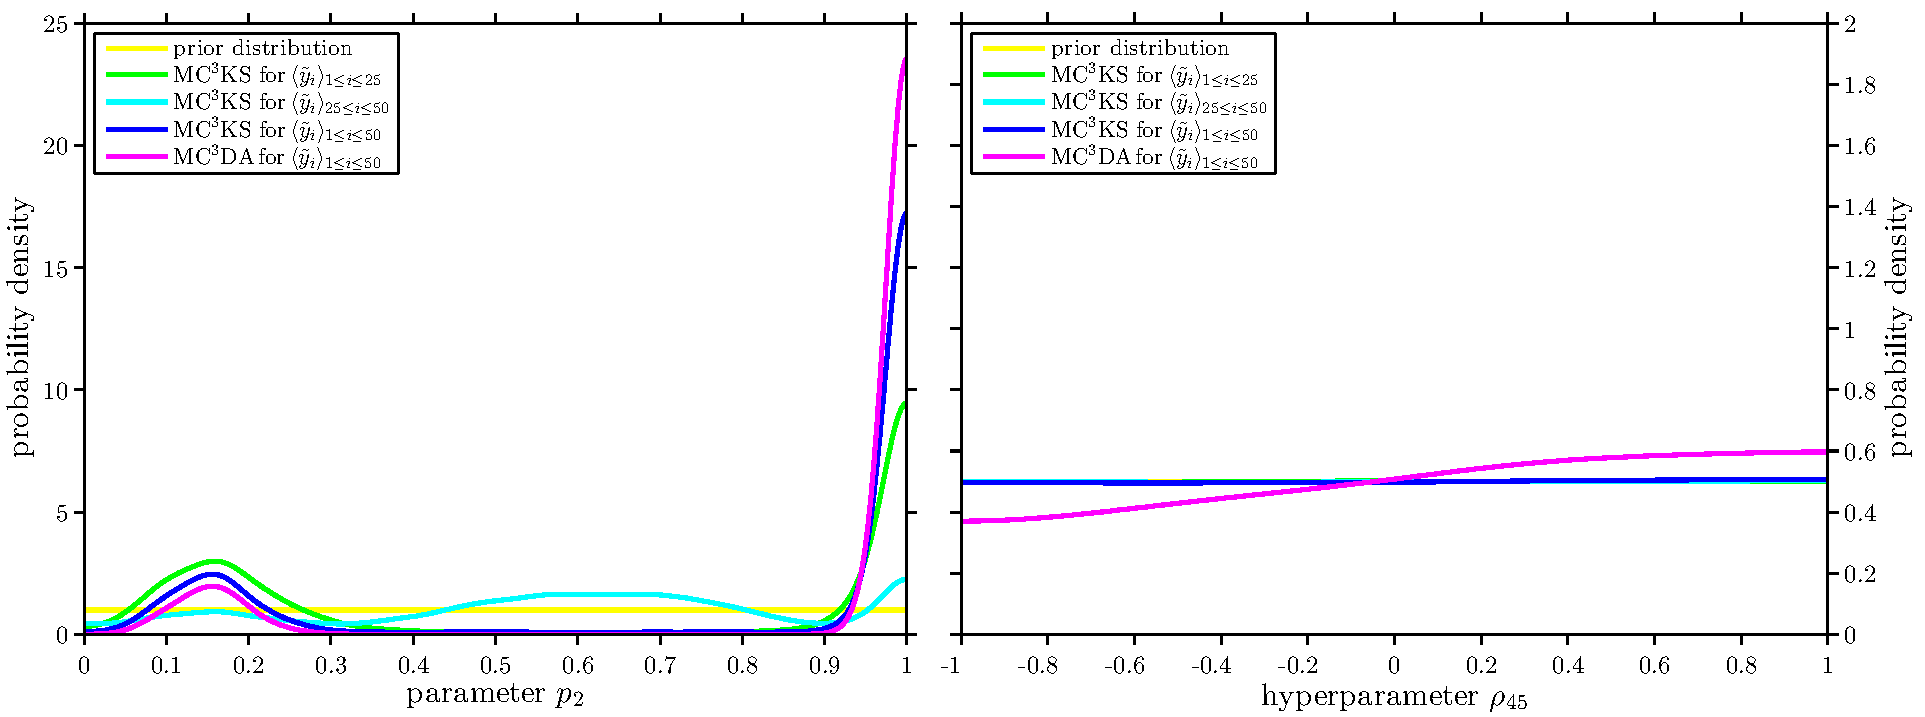
\includegraphics[width=\JAISfigWidth]{fig_JAIS_KSDA_1D_Param2Rho45}
  \caption[Posterior marginals of \(p_2\) and \(\rho_{45}\)]{Posterior marginals of \(p_2\) and \(\rho_{45}\).
           Analyzing \(\tuple{\perfect{y}_i}_{1 \leq i \leq 50}\) by \(\text{MC}^3\text{KS}\) reveals two separated posterior modes in the posterior of \(p_2\).
           As expected the posterior of the correlation hyperparameter \(\rho_{45}\) is flat and uninformative.
           Slightly more pronounced posterior structures are discovered by \(\text{MC}^3\text{DA}\).
          }
  \label{res:JAIS:Param2Rho45}
\end{figure}
% \mu_4, \sigma^2_4
\begin{figure}[p]
  \centering
  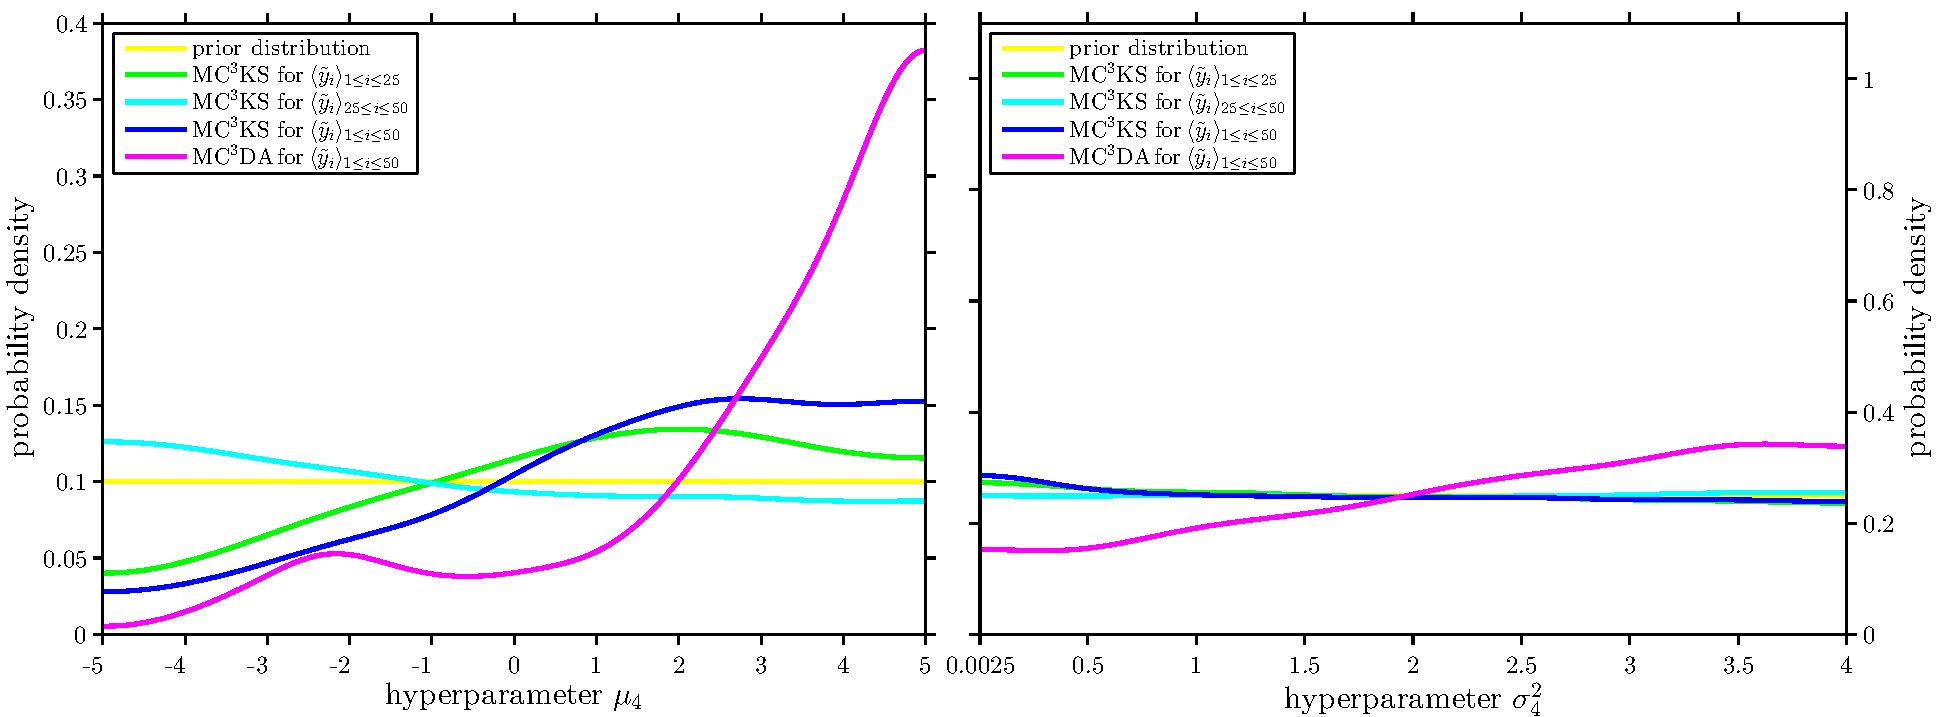
\includegraphics[width=\JAISfigWidth]{fig_JAIS_KSDA_1D_Hyper4}
  \caption[Posterior marginals of \(\mu_4\) and \(\sigma^2_4\)]{Posterior marginals of \(\mu_4\) and \(\sigma^2_4\).
           Both the posterior marginals of \(\mu_4\) and \(\sigma^2_4\) that were sampled by \(\text{MC}^3\text{KS}\) are rather flat and uninformative.
           On the contrary, the posterior of \(\mu_4\) explored by \(\text{MC}^3\text{DA}\) features more definite structure.
          }
  \label{res:JAIS:Hyper4}
\end{figure}
% \mu_5, \sigma^2_5
\begin{figure}[p]
  \centering
  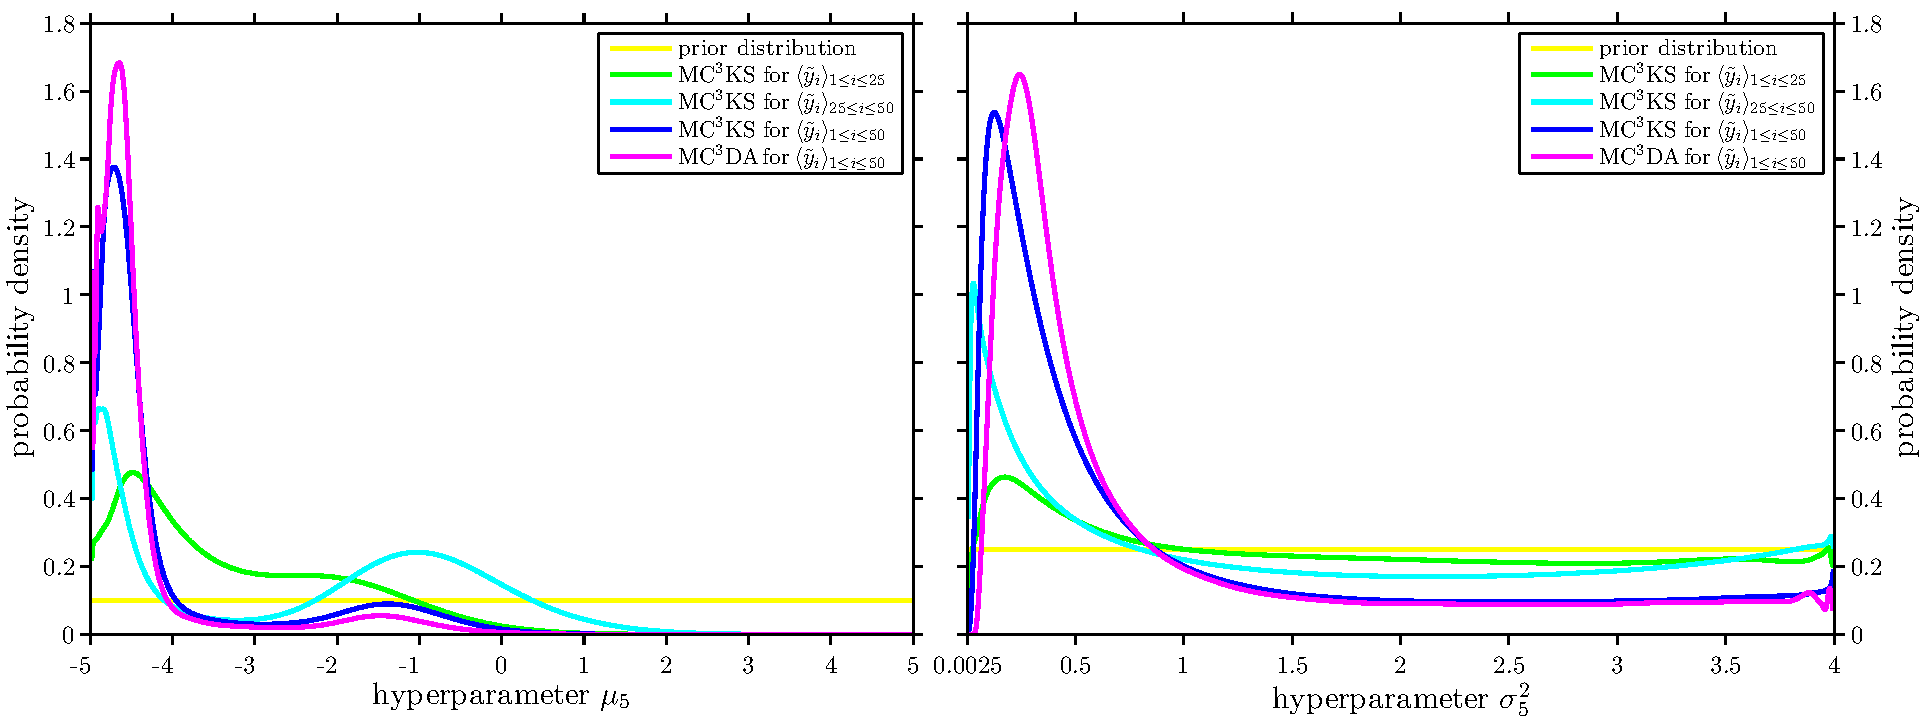
\includegraphics[width=\JAISfigWidth]{fig_JAIS_KSDA_1D_Hyper5}
  \caption[Posterior marginals of \(\mu_5\) and \(\sigma^2_5\)]{Posterior marginals of \(\mu_5\) and \(\sigma^2_5\).
           The posterior marginals of \(\mu_5\) and \(\sigma^2_5\) feature a distinctive structure as compared to the priors.
           The posterior of \(\mu_5\) is multimodal whereas the one of \(\sigma^2_5\) is unimodal.
           With respect to the posteriors sampled by \(\text{MC}^3\text{KS}\), the ones that are due to \(\text{MC}^3\text{DA}\) are slightly more evolved in structure.
          }
  \label{res:JAIS:Hyper5}
\end{figure}
% 2D: \((\mu_1,\sigma_1^2)\) and \((\mu_1,\mu_4)\)
\begin{figure}[p]
  \centering
  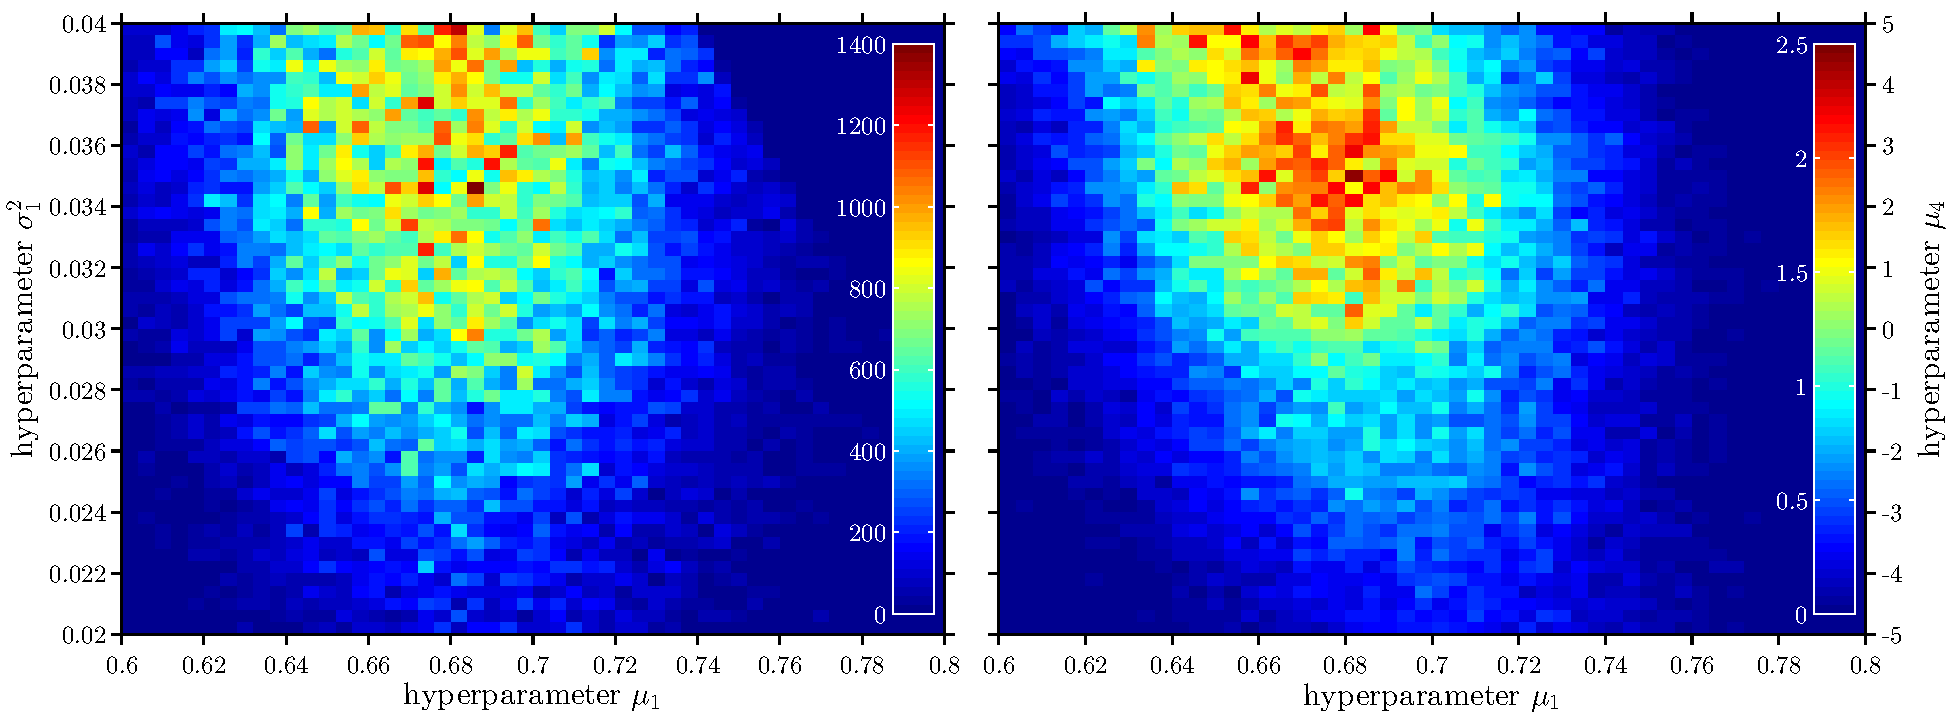
\includegraphics[width=\JAISfigWidth]{fig_JAIS_KS_2D_Mean1Sigma1Mean4}
  \caption[2D posteriors of \((\mu_1,\sigma_1^2)\) and \((\mu_1,\mu_4)\)]{2D posteriors of \((\mu_1,\sigma_1^2)\) and \((\mu_1,\mu_4)\).
           Two-dimensional posterior projections for analyzing \(\tuple{\perfect{y}_i}_{1 \leq i \leq 50}\) by \(\text{MC}^3\text{KS}\) are shown for \((\mu_1,\sigma_1^2)\) and \((\mu_1,\mu_4)\).
           A small dependency structure in the posteriors can be seen.
           Linear Pearson coefficients of correlation are found as \(r_{\mu_1,\sigma_1^2} = -0.08\) and \(r_{\mu_1,\mu_4} = -0.22\).
          }
  \label{res:JAIS:2D:Mean1Sigma1Mean4}
\end{figure}
% 2D: \((\mu_5,\mu_1\) and \((\mu_5,\mu_4)\)
\begin{figure}[p]
  \centering
  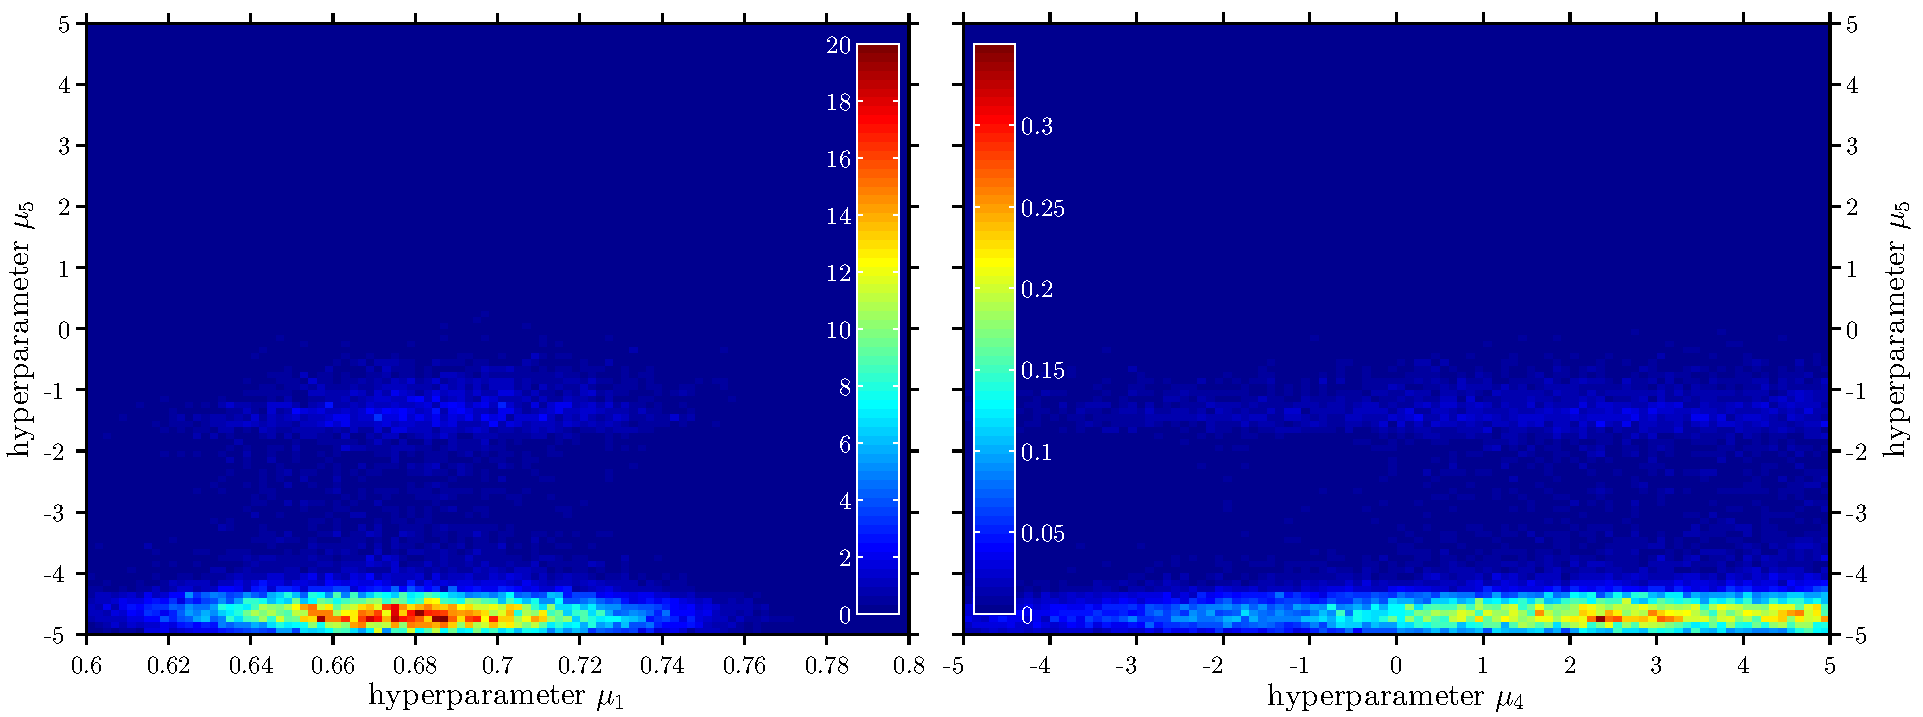
\includegraphics[width=\JAISfigWidth]{fig_JAIS_KS_2D_Mean5Mean1Mean4}
  \caption[2D posteriors of \((\mu_1,\mu_5)\) and \((\mu_4,\mu_5)\)]{2D posteriors of \((\mu_1,\mu_5)\) and \((\mu_4,\mu_5)\).
           For \((\mu_1,\mu_5)\) and \((\mu_4,\mu_5)\) two-dimensional posterior projections are shown that are due to analyzing \(\tuple{\perfect{y}_i}_{1 \leq i \leq 50}\) with \(\text{MC}^3\text{KS}\).
           The corresponding posteriors do not feature any marked dependency structure.
          }
  \label{res:JAIS:2D:Mean5Mean1Mean4}
\end{figure}

\subsection{Final results}
% FINAL RESULTS
First of all we jointly analyze the total data \(\tuple{\perfect{y}_i}_{1 \leq i \leq 50}\).
For \(N=10^5\) iterations of the \(\text{MC}^3\text{KS}\) algorithm the total program runtime amounts to \(t \approx \unit[30]{h}\) on a single core.
% ACCEPTANCE RATES
Blockwise acceptance rates were found to be ca.\ \(\unit[20]{\%}\) for \((p_2)\), \(\unit[40]{\%}\) for \((\mu_1,\sigma^2_1)\),
\(\unit[60]{\%}\) for \((\mu_4,\sigma^2_4,\rho_{45})\) and \(\unit[10]{\%}\) for \((\mu_5,\sigma^2_5)\).
% BETA VIOLATIONS
With \cref{eq:JAIS:Beta:Transform2Stat} a number of \(10327\) blockwise proposals \((\mu_1,\sigma^2_1)\) had been rejected because of violating the prior requirement \(\alpha_1,\beta_1>1\).
% POSTERIOR MARGINALS
Marginal posterior densities of the QoI are shown in \cref{res:JAIS:Hyper1,res:JAIS:Param2Rho45,res:JAIS:Hyper4,res:JAIS:Hyper5}.
% BOUNDARY CORRECTION
Based on appropriate boundary correction methods, the densities shown have been obtained by kernel smoothing of the MCMC posterior samples.
% POSTERIOR FIDELITY
Following precursory discussions we attribute an acceptable degree of fidelity to the posteriors obtained.
We are confident that we have revealed a ``good'' approximation of the true posteriors, regardless of whether some of them are flat and only weakly informative.
\par % DATA CONFIGURATIONS
We also analyze the data subconfigurations \(\tuple{\perfect{y}_i}_{1 \leq i \leq 25}\) and \(\tuple{\perfect{y}_i}_{26 \leq i \leq 50}\) separately.
The posterior densities produced by separate analyses may differ considerably.
% REPRESENTATIVENESS
With respect to the posteriors yielded by analyzing \(\tuple{\perfect{y}_i}_{1 \leq i \leq 50}\), the two data subconfigurations are representative to a different degree.
% CONCLUSION
Those findings indicate that \(n=25\) is a comparably low number of observations while \(n=50\) is moderately satisfying for the Bayesian calibration of mean hyperparameters and the forward model parameter.
Properly identifying the variance and correlation hyperparameters would require a higher number of observations.
This is hardly surprising regarding the complex uncertainty setup, the number of unknowns, the unknown character of the forward model, and the inverse nature of the calibration problem.
\par % INTERPRETATION: CLASSICAL INVERSION & DISTRIBUTION FITTING
At this point it is important to mention that multilevel model calibration shares and combines aspects of classical inverse problems,
i.e.\ the inference of an unknown constant forward model parameter, and direct sample statistics, i.e.\ fitting a parametric distribution to a random data sample.
Thereby Bayesian multilevel model calibration also inherits the usual difficulties inherent in inversion and distribution fitting.
\par % DISCUSSION: HYPER1
The marginal posteriors of \(\mu_1\) and \(\sigma^2_1\) are shown in \cref{res:JAIS:Hyper1}.
In comparison to the prior, the posterior of \(\mu_1\) shows a pronounced structure.
Separately analyzing \(\tuple{\perfect{y}_i}_{1 \leq i \leq 25}\) and \(\tuple{\perfect{y}_i}_{26 \leq i \leq 50}\) gives rise to two different posterior modes.
Those are suggested by the corresponding experiment-specific realizations \(\tuple{p_{1,i}}_{1 \leq i \leq 25}\) and \(\tuple{p_{1,i}}_{26 \leq i \leq 50}\).
A joint analysis of \(\tuple{\perfect{y}_i}_{1 \leq i \leq 50}\) leads to a mode that lies in between the two abovementioned ones.
The posterior marginal of the spread hyperparameter \(\sigma^2_1\) is comparably structureless and therefore less informative.
% DISCUSSION: PARAM2 & RHO45
In \cref{res:JAIS:Param2Rho45} the posterior marginals of \(p_2\) and \(\rho_{45}\) are depicted.
Due to the fact that data subconfigurations \(\tuple{\perfect{y}_i}_{1 \leq i \leq 25}\) and \(\tuple{\perfect{y}_i}_{26 \leq i \leq 50}\)
are to a different degree informative about further unknowns, e.g.\ about \((\mu_1,\sigma^2_2)\) which was discussed above, the posteriors obtained for the constant model parameter \(p_2\) may deviate as well.
The analysis of \(\tuple{\perfect{y}_i}_{1 \leq i \leq 50}\) by \(\text{MC}^3\text{KS}\) reveals two clear and separated posterior modes in the posterior of the forward model parameter \(p_2\),
whereas the posterior of the correlation hyperparameter \(\rho_{45}\) is flat.
This is according to our previous expectations.
% DISCUSSION: HYPER4
Posteriors of \(\mu_4\) and \(\sigma^2_4\) are given in \cref{res:JAIS:Hyper4}.
That they are comparably flat and uninformative prevents from drawing clear inferential conclusions.
% DISCUSSION: HYPER5
This statement does not hold for the posteriors of \(\mu_5\) and \(\sigma^2_5\) that can be seen in \cref{res:JAIS:Hyper5}.
While the former features a bimodal structure and drops to zero for higher values of \(\mu_5\), the latter is unimodal and reaches a nonzero ``plateau'' for higher values of \(\sigma^2_5\).
Since this region accumulates considerable posterior probability mass, one cannot exclude those values of \(\sigma^2_5\).
% DATA AUGMENTATION
Apart from the results of \(\text{MC}^3\text{KS}\) the figures \cref{res:JAIS:Hyper1,res:JAIS:Param2Rho45,res:JAIS:Hyper4,res:JAIS:Hyper5} also contain the results of analyzing \(\tuple{\perfect{y}_i}_{1 \leq i \leq 50}\)
by \(\text{MC}^3\text{DA}\), i.e.\ an alternative algorithm which is based on data augmentation.
This technique will be further detailed in \cref{sec:JAIS:Augmentation}.
\par % EPISTEMIC INTERVALS
Note that Bayesian probabilities feature a richer structure than mere epistemic intervals.
% INTERPRETATION
Conforming with a subjective Bayesian paradigm, probabilities are identified as relative degrees of belief or plausibility.
Thus multivariate probability distributions, that may contain complex dependency structures
and that are not entirely defined by their marginals only, have to be interpreted accordingly.
% POSTERIOR CORRELATION
The marginal densities shown hide this possibly existing posterior correlations.
We provide a selection of two-dimensional posterior projections in \cref{res:JAIS:2D:Mean1Sigma1Mean4,res:JAIS:2D:Mean5Mean1Mean4}.
\par % DETAILED DISCUSSION
Parameters that were assumed to be statistically independent a priori,
e.g.\ the parameter \(p_2\), the hyperparameters \(\bm{\theta}_1\) and the hyperparameters \(\bm{\theta}_{45}\),
can be statistically dependent a posteriori.
Small negative correlations in the posteriors of \((\mu_1,\sigma^2_1)\) and \((\mu_1,\mu_4)\) shown in \cref{res:JAIS:2D:Mean1Sigma1Mean4,res:JAIS:2D:Mean5Mean1Mean4},
with linear Pearson coefficients of correlation \(r_{\mu_1,\sigma^2_1} = -0.08\) and \(r_{\mu_1,\mu_4} = -0.22\) were discovered, respectively.
% CREDIBLE INTERVALS
In order to provide final results of interval-like character one could define suitable Bayesian credible intervals or sets that accumulate a certain proportion, e.g.\ \(\unit[95]{\%}\), of the total posterior mass.
However, the definition of such intervals is ambiguous and would still bear the probabilistic interpretation, therefore we refrain from defining Bayesian credible intervals.

\subsection{First conclusion}
% ACHIEVEMENTS
With the proposed \(\text{MC}^3\text{KS}\) algorithm the Bayesian formulation of the challenge problem could be solved.
% POTENTIAL IMPROVEMENTS
The numerical efficiency of the MCMC sampling scheme, that was based on independently sampling from the priors, could be easily increased.
Obtained posteriors could be approximated by suitable distributions that are easy to sample.
Utilizing these as proposal distributions would lead to higher acceptance rates and better mixing properties.
% PARALLELIZATION
Most Bayesian computations can only be parallelized by running several Markov chains simultaneously.
An obvious parallelization strategy for the devised algorithm is to parallelize the estimation of the transformed likelihood on the level of forward model runs.
This also suggests the possibility of studying the posterior for significantly larger \(K\) and smaller \(h\).
% KERNEL SMOOTHHING
Moreover different classes of kernel functions \(\mathcal{K}\), e.g.\ with bounded nonzero support,
or more advanced KDE techniques, e.g.\ locally adaptive schemes or other bias reduction and correction methods, could be employed.
% SHORTCOMINGS
The major shortcoming of the approach was the dependency of the final results on free algorithmic tuning parameters.
Parameter tuning had to be based on heuristic criteria and plausibility checks and the fidelity of the final posteriors could only be provisionally assessed.
% OUTLOOK
In the following section we will therefore propose a complementary multilevel approach that aims at enhancing the level of posterior fidelity.
